%%%%%%%%%%%%%%%%%%%%%%%%%%%%%%%%%%%%%%%%%%%%%%%%%%%%%%%%%%%%%%%%%%%%%%%%%%%%%%%
%%%%%%%%%%%%%%%%%%%%%%%%%%%%%%%%%%%%%%%%%%%%%%%%%%%%%%%%%%%%%%%%%%%%%%%%%%%%%%%
% APPENDIX
%%%%%%%%%%%%%%%%%%%%%%%%%%%%%%%%%%%%%%%%%%%%%%%%%%%%%%%%%%%%%%%%%%%%%%%%%%%%%%%
%%%%%%%%%%%%%%%%%%%%%%%%%%%%%%%%%%%%%%%%%%%%%%%%%%%%%%%%%%%%%%%%%%%%%%%%%%%%%%%
\newpage
\appendix
\onecolumn
\large
\begin{center}
   \emph{Appendix of paper ``In-Context Decision Transformer: Reinforcement Learning via Hierarchical Chain-of-Thought"} 
\end{center} 
\normalsize

\section{Pseudocode of In-context Decision Transformer}
\label{appendix A}

\begin{algorithm}[h!]
\caption{In-context Decision Transformer.}
\label{IDT algorithm}
\begin{algorithmic}[1]
\STATE \textbf{Input:} A dataset of Trajectories, Max Iterations $M$ as training phase, Max episodes $m$ at testing phase, A number of trajectories $n$ in hierarchical chain of experience, A number of steps of low-level actions $c$ for one high-level decision
\STATE \textbf{Output:} The generated low-level actions
\STATE // \textbf{Training}
\FOR{$i=1$ $\textbf{to}$ $M$}
    \STATE Randomly sample $n$ episodes from dataset $s=(\tau^{1},\tau^{2},\dots,\tau^{n})$
    \STATE Sort $n$ episodes ascending according to their returns $\sum_{t=0}^T{r_t^1}\leq\sum_{t=0}^T{r_t^2}\leq\dots\leq\sum_{t=0}^T{r_t^n}$
    \STATE Compute returns-to-go $\hat{R}_t=\hat{R}_0-\sum_{j=0}^tr_j$ for all steps for each episode, where $\hat{R}_0=\sum_{t=0}^T{r_t^n}$
    \STATE The Reviewing Decisions module encodes a high-level decisions $\textbf{z}$ every $c$ steps
    \STATE Concatenate $n$ episodes as a high-level sequence $s_h=(\tau_h^{1},\tau_h^{2},\dots,\tau_h^{n})$ based on Equation~\eqref{hcoe}
    \STATE Build a low-level sequence every $c$ steps based on Equation~\eqref{lcoe}
    \STATE The Making Decisions module predicts the next high-level decision tokens, and then the Decision to Go module predicts the next $c$ steps low-level action tokens for each predicted high-level decision token
    \STATE Train the Reviewing Decisions, Making Decisions, and Decision to Go modules based on the loss of predicted low-level actions end-to-end    
\ENDFOR
\STATE // \textbf{Testing}
\FOR{$i=1$ $\textbf{to}$ $m$}
    \STATE Start a new episode $i$ and reset the timestep $t=0$
    \WHILE{$t\leq T$}
        \STATE The Making Decisions model generates next high-level decision token $\textbf{z}_t^i$ based on the across-episodic context $(\tau_h^{i-3},\tau_h^{i-2},\tau_h^{i-1},\dots,\hat{R}_t^i,o_t^i)$, where $\tau_h^{i}$ is expressed as Equation~\eqref{hcoe}
        \FOR{$k=0$ $\textbf{to}$ $c-1$}
            \STATE The Decisions to Go model generates next low-level action $a_{t+k}^i$ based on the previous context $(\textbf{z}_t^i,o_t^i,a_t^i,r_t^i,\dots,\textbf{z}_{t}^i,o_{t+k}^i)$
        \ENDFOR
        % \STATE The Decisions to Go model generates next $c$ steps low-level actions $(a_t^i,\dots,a_{t+c-1}^i)$, where the generated low-level sequence is express as $(\textbf{z}_t^i,o_t^i,a_t^i,r_j^i,\dots,\textbf{z}_{t}^i,o_{t+c-1}^i,a_{t+c-1}^i,r_{t+c-1}^i)$
        \STATE The Review Decisions model encode the executed decision $\textbf{z}_t^i$ from the $c$ steps $(o_t^i,a_t^i,\dots,o_{t+c-1}^i,a_{t+c-1}^i)$
        \STATE Compute the sum of $c$ steps rewards $\hat{r}_t^i$ and the next returns-to-go $\hat{R}_{t+c}^i$
        \STATE Receive the next observation $o_{t+c}^i$
        \STATE Update the across-episodic context $((\tau_h^{i-3},\tau_h^{i-2},\tau_h^{i-1},\dots,\hat{R}_t^i,o_t^i,\textbf{z}_t^i,\hat{r}_t^i,d_t^i,\hat{R}_{t+c}^i,o_{t+c}^i)$
        \STATE Update time step $t = t+c$
    \ENDWHILE
\ENDFOR
\end{algorithmic}
\end{algorithm}

In Algorithm~\ref{IDT algorithm}, we introduce the training and testing process of IDT. At each iteration, we first construct a sequence consisting of high-level decisions, as described in lines 5-9. Importantly, high-level decisions in the dataset are encoded by the Reviewing Decisions module (line 8). In addition, each high-level decision will correspond to a short sequence of $c$ steps low-level actions, as described in line 10. Based on the constructed sequences, the Making Decisions and Decisions to Go modules predict high-level decisions and low-level actions, respectively (line 11). Finally, the low-level actions are evaluated with either cross-entropy loss or mean-squared error, depending on whether the actions are discrete or continuous. The losses from each time step are averaged and updated in all three modules end-to-end, as described in line 12.

During testing, IDT needs to generate low-level actions autoregressively and interact with the environment $m$ episodes. At step $t$ of episode $i$ (line 18), the Making Decisions module first generates a high-level decision token $\textbf{z}_t^i$ conditioned on the across-episodic context $(\tau_h^{i-3},\tau_h^{i-2},\tau_h^{i-1},\dots,\hat{R}_t^i,o_t^i)$, where $\tau_h^{i}$ is expressed as Equation~\eqref{hcoe}. Then, the Decision to Go will generate the following $c$ steps low-level actions $(a_t,\dots,a_{t+c-1})$ autoregressively, as described in lines 19-21. Unlike training, the Reviewing Decisions module encodes the executed decision from the actions generated by the Decision to Go module. Then, it serves as a condition for generating the next high-level decision $\textbf{z}_{t+c}^i$, as described in lines 22-26.

\section{Experimental Details}
\label{appendix B}

Source code is available at \href{https://github.com/SiliHuang-ai/IDT}{here}.

\noindent\textbf{Compute.}
Experiments are carried out on NVIDIA GeForce RTX 3090 GPUs and NVIDIA A10 GPUs.
Besides, the CPU type is Intel(R) Xeon(R) Gold 6230 CPU @ 2.10GHz.
Since our memory is not enough to support AT training in D4rl tasks, we refer to the results of the original paper. In contrast, our method has lower memory requirements because it naturally shortens the across-episodic contexts.

\noindent\textbf{Hyperparameters.}
The default length of across-episodic is four trajectories unless mentioned otherwise. In D4RL and Large Grid World, the Decisions to Go module generates $c=10$ steps low-level actions while the Making Decisions module generates one high-level decision. In conventional Grid World, we set $c=5$ because the task is too short. Except for independent parameters and different input and output dimensions, three modules in IDT follow the same architecture. In summary, Table~\ref{hyper} shows the hyperparameters used in our IDT model.

\begin{table}[t]
\centering
\caption{Hyperparameters of IDT.}
\resizebox{0.8\textwidth}{!}{
\begin{tabular}{@{}l|l|l@{}}
\toprule
 & Hyperparameters & Value \\ \midrule
 & Number of layers & 3 \\
 & Number of attention heads & 3 \\
 & Embedding dimension & 128 \\
 & Activation function & ReLU \\ 
 & $c$ steps controlled by one high-level decision & 10 D4RL and Large Grid World \\
 &  & 5 Grid World \\ \midrule
\multirow{7}{*}{Training}& Batch size & 64 \\
 & Dropout & 0.1 \\
 & Learning rate & 1e-4 \\
 & Learning rate decay & Linear warmup for 1e5 steps \\ 
 & Grad norm clip & 0.25 \\
 & Weight decay & 1e-4 \\
 & Number of trajectories to form across-episodic contexts $n$ & 4 (Large) Dark Key-to-Door \\
 &  & 10 other tasks in Grid World \\
 &  & 4 D4RL \\ \midrule
\multirow{14}{*}{Testing} & Target return for HalfCheetah & 12000 \\
 & Target return for Hopper & 3600 \\
 & Target return for Walker & 5000 \\
 & Target return for Darkroom & 20 \\
 & Target return for Darkroom Hard & 1 \\
 & Target return for Darkroom Dynamic & 20 \\
 & Target return for Darkroom Key-to-Door & 2 \\
 & Target return for Large Darkroom & 15 \\
 & Target return for Large Darkroom Hard & 1 \\
 & Target return for Large Darkroom Dynamic & 15 \\
 & Target return for Large Darkroom Key-to-Door & 2 \\
 & Number of trajectories to form across-episodic contexts $n$ & 4 (Large) Dark Key-to-Door \\
 &  & 10 other tasks in Grid World \\
 &  & 4 D4RL \\ 
 \bottomrule
\end{tabular}
}
\label{hyper}
\end{table}

\section{Additional Experimental Results}
\label{additional experiments}

\begin{figure}
    \centering
    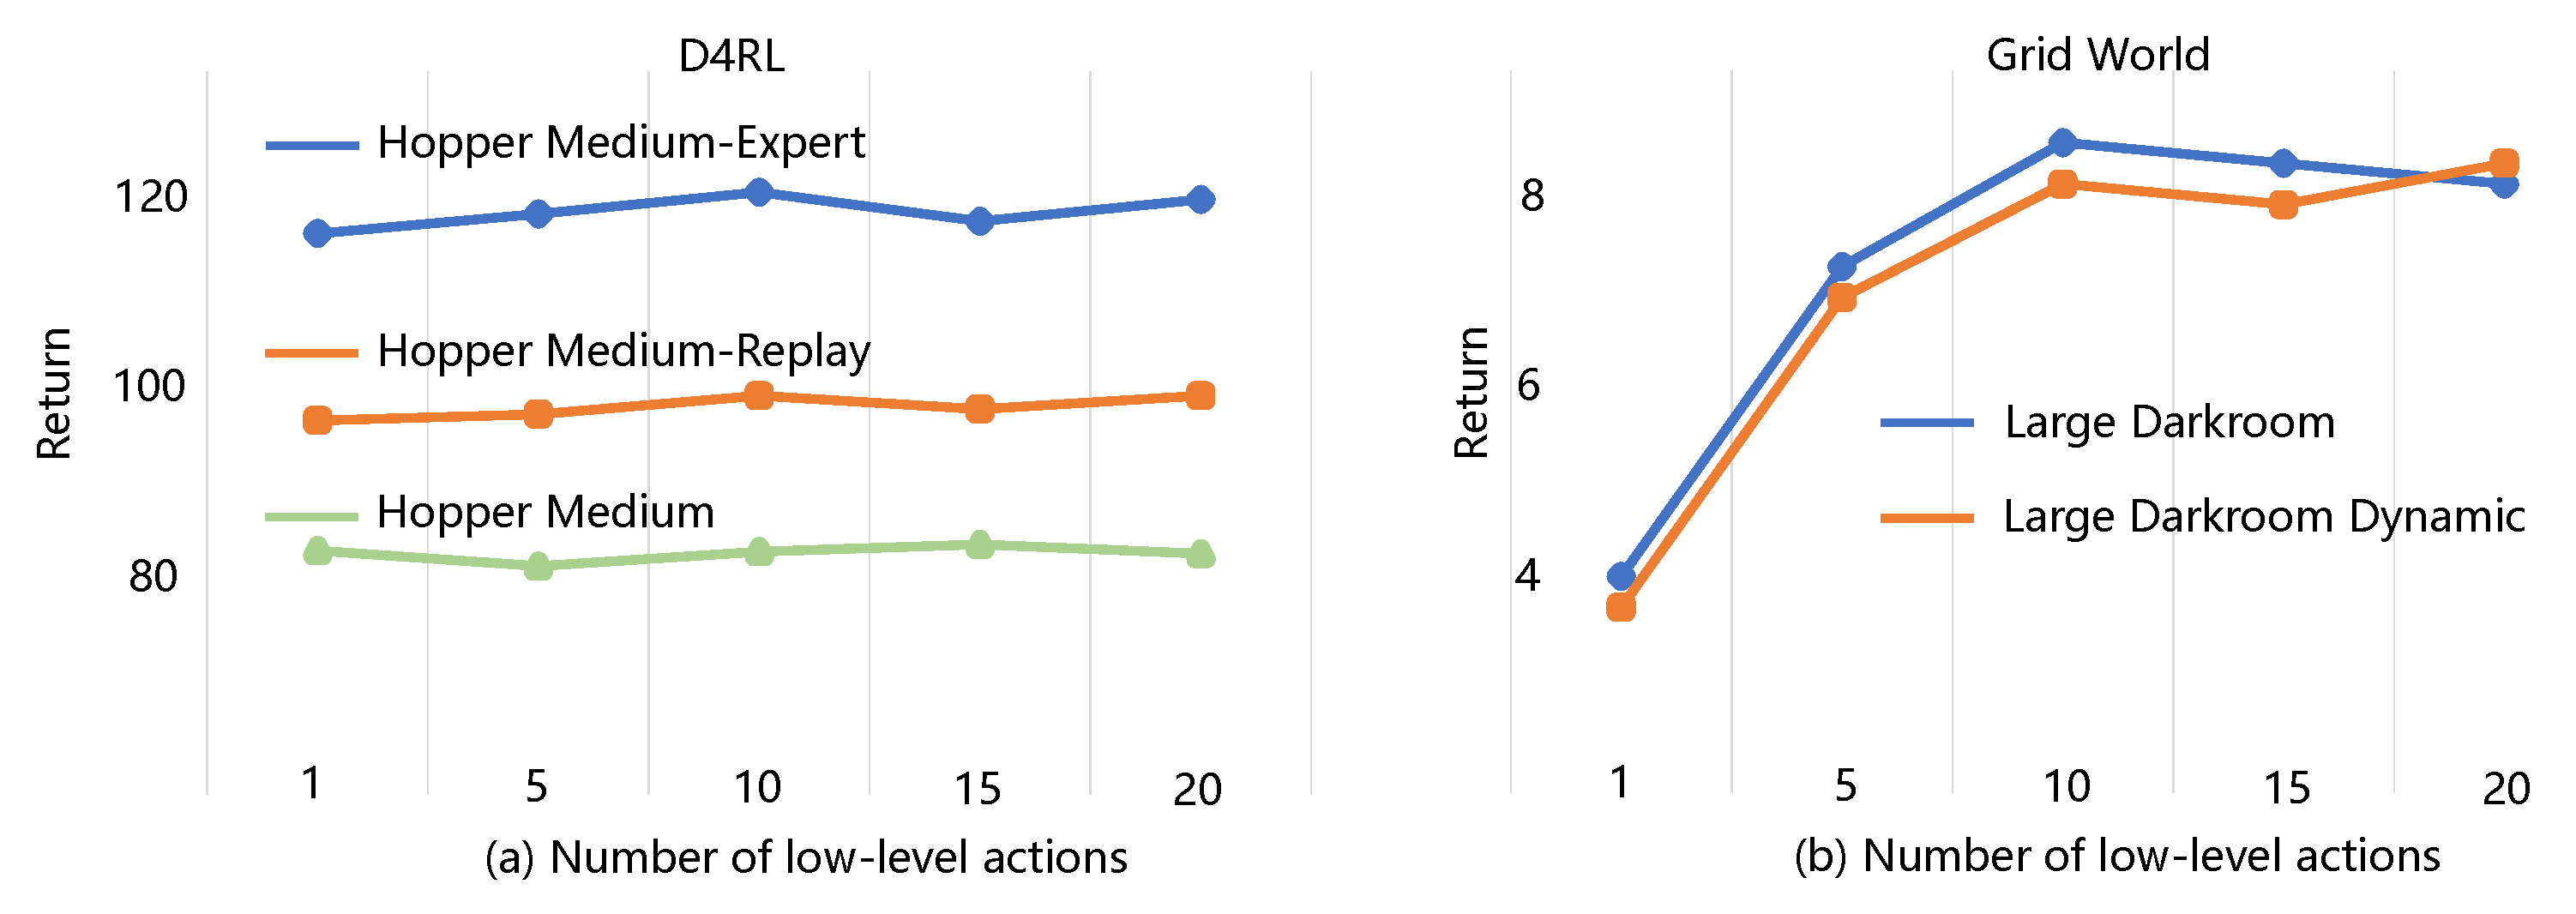
\includegraphics[width=0.8\columnwidth]{results/horizon.pdf}
    \caption{Parameter sensitive analysis of $c$. (a) IDT maintains stable performance to changes in $c$ in dense reward D4RL tasks. (b) As $c$ increases, it becomes easier for the model to receive positive feedback to discover the target location in sparse reward Grid World tasks.}
    \label{horizon}
\end{figure}

\begin{figure}
    \centering
    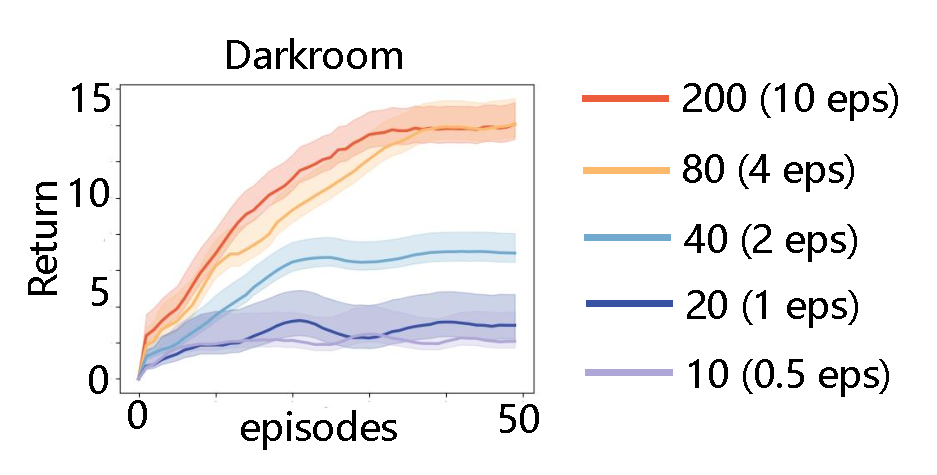
\includegraphics[width=0.5\columnwidth]{results/context_window.pdf}
    \caption{Context size: IDT in Darkroom with different context sizes. IDT emerges with trial-and-error ability once the context size is large enough and across-episodic.}
    \label{Context size}
\end{figure}

\begin{table*}
\caption{Results for training and testing times. We report the training time per 10k gradient updates, the testing time for 50 episodes over Grid World, and 10 episodes over D4RL. As the task length increases, the context length is forced to grow exponentially, resulting in a square increase in computational costs. In contrast, IDT completes trial-and-error on high-level decisions in sizes smaller than one episode length, significantly reducing computational costs.
}
\begin{center}
\resizebox{0.9\textwidth}{!}{
\begin{tabular}{l|l|rrr|rrr}
\toprule
\specialrule{0em}{1.0pt}{1.0pt}
\toprule
\multirow{2}{*}{Context size (step)}&\multirow{2}{*}{Tasks} & \multicolumn{3}{c|}{Training (hour)} & \multicolumn{3}{c}{Testing (minute)} \\ 
\cline{3-8}
 & & AT & AD & Ours & AT & AD & Ours \\ 
 \toprule
\multirow{4}{*}{200} & Darkroom & 0.27 & 0.23 & 0.21 & 0.62 & 0.61 & 0.65 \\ % 25x10
& Darkroom Hard & 0.29 & 0.28 & 0.20 & 0.59 & 0.56 & 0.58 \\ % 25x10
& Darkroom Dynamic & 0.33 & 0.31 & 0.21 & 0.65 & 0.62 & 0.67 \\ % 25x10
& Dark Key-to-Door & 1.12 & 1.01 & 0.44 & 1.89 & 1.50 & 1.52 \\ % 50x10
\toprule
\multirow{4}{*}{2000} & Large Darkroom & 5.09 & 4.70 & 2.49 & 67.22 \scriptsize{(13$\times$)} & 45.08 \scriptsize{(9$\times$)} & 5.27 \\ % 200x10
& Large Darkroom Hard & 6.48 & 6.69 & 2.93 & 66.81 \scriptsize{(11$\times$)} & 44.96 \scriptsize{(7$\times$)} & 6.09 \\ % 200x10
& Large Darkroom Dynamic & 5.71 & 5.84 & 2.73 & 62.06 \scriptsize{(11$\times$)} & 42.12 \scriptsize{(8$\times$)} & 5.51 \\ % 200x10
& Large Dark Key-to-Door & 18.87 & 18.23 & 3.06 & 167.07 \scriptsize{(27$\times$)} & 76.79 \scriptsize{(12$\times$)} & 6.18 \\
\toprule
\multirow{3}{*}{4000} & HalfCheetah & 36.18 & 37.10 & 21.90 & 234.20 \scriptsize{(37$\times$)} & 173.11 \scriptsize{(28$\times$)} & 6.29 \\
& Walker & 32.82 & 33.77 & 20.08 & 233.18 \scriptsize{(36$\times$)} & 172.34 \scriptsize{(26$\times$)} & 6.51 \\
& Hopper & 24.08 & 22.23 & 12.99 & 232.82 \scriptsize{(35$\times$)} & 172.92 \scriptsize{(26$\times$)} & 6.56 \\
\toprule
\specialrule{0em}{1.0pt}{1.0pt}
\toprule
\end{tabular}
}
\end{center}
\label{cost}
\end{table*}



\noindent\textbf{Parameter Sensitive Analysis of $c$.}~~
An important insight of IDT is that one high-level decision can guide $c$-step low-level actions. We aim to investigate whether the size of $c$ will affect the performance of IDT. Therefore, we tested $c=1,5,10,15,20$ in D4RL and Grid World, respectively. As shown in Figure~\ref{horizon}, IDT maintains stable performance to changes in $c$ in D4RL tasks. In contrast, larger $c$ achieves better performance in Grid World. This is because the Grid World is designed for tasks with sparse rewards where the agent needs to rely on rewards to reason about the target location. As $c$ increases, it becomes easier for the model to receive positive feedback to discover the target location.

\noindent\textbf{What Context Size is Required for IDT?} Similar to other in-context RL methods, we also test how context sizes are required for IDT emerging with trial-and-error ability. As shown in Figure~\ref{Context size}, multi-episodic contexts of 4 episodes are necessary to learn a near-optimal IDT. When the context size is roughly the length of an episode, IDT begins to emerge with self-improvement. The reason for this is likely that the context is large enough to retrain across-episodic information – e.g., at the start of a new episode, the context will be filled with transitions from most of the previous episode.



